This section describes the design of our system, first with a system overview
and then with more in-depth information about our tabs.
\subsection{How our web application works}
%figure x5
\begin{figure}[h]
\centering
\includegraphics[width=1\textwidth]{web_system_backboneWebapp.png}
\caption{\label{fig:web_system_backboneWebapp}A general build of a backbone web-app.}
\end{figure}

\refer{fig:web_system_backboneWebapp} shows how a backbone\cite{web_1} web application works in general. We have a user, that interacts with a browser. A browser renders the DOM of our web application. How it does this is up to the browser. Different browsers might display it differently. Models and Collections will talk to the server to update themselves. For example, our \textit{Experiments} collection will retrieve experiments from the server and update itself with a call to it’s fetch() method. Out of the components that go into this figure, we are in charge of and only capable of changing a few of these; \textbf{View}, \textbf{Template}, \textbf{Collection} and \textbf{Model}. See the Backbone section of Frameworks in section \ref{sec:web_frame} more information.

\subsection{System overview}
%figure 2
\begin{figure}[h]
\centering
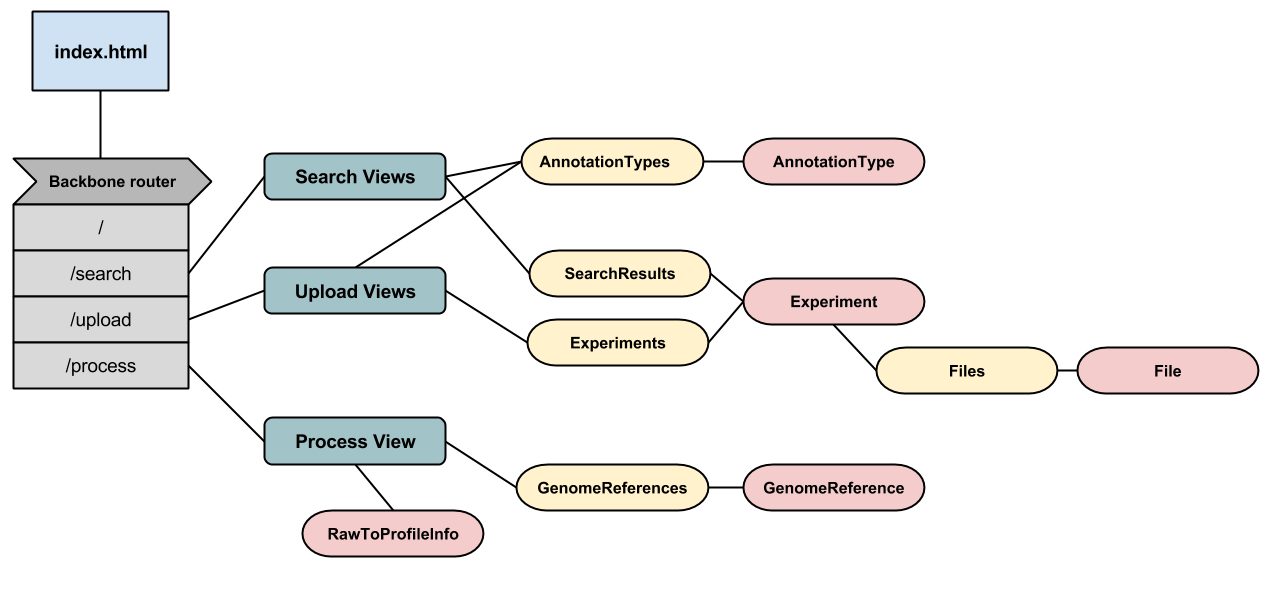
\includegraphics[width=1\textwidth]{web_system_overview.png}
\caption{\label{fig:web_system_overview}Overview of the relations between the different JavaScript prototypes in the system.}
\end{figure}

Since our app is built using Backbone\cite{web_1}, our app is divided into the parts \textbf{Misc}, \textbf{Views}, \textbf{Collections} and \textbf{Models}. In \refer{fig:web_system_overview}, we can see the system overview. The \textbf{views} are the parts in green, the \textbf{collections} the parts in yellow and the \textbf{model} the parts in red. The parts in grey represent the router which belongs in our Misc category. It is responsible for rerouting links. For example, when a user clicks the search tab, the router navigates to /search, but instead of loading the whole /search over the page we are currently on, our router will open our search tab below our navigation bar. The \textbf{Misc} category also holds our Main.js, which is in charge of setting up and starting the app.

\subsection{Search}
The search tab has three views, the main one being \textit{Search}, which acts as a container for the \textit{SearchResultsView}and holds the search input field and the various buttons displayed. The \textit{SearchResultsView} handles rendering the annotations and the \textit{ExperimentViews}, where one \textit{ExperimentView} is created for every experiment returned from a search. The actual data retrieved is stored, by experiment, in \textit{Experiment models}. To organize this data, we have a collection to contain all the experiments retrieved, called \textit{SearchResults}.
 
%figure bla bla/lalalallala
\begin{figure}[h]
\centering
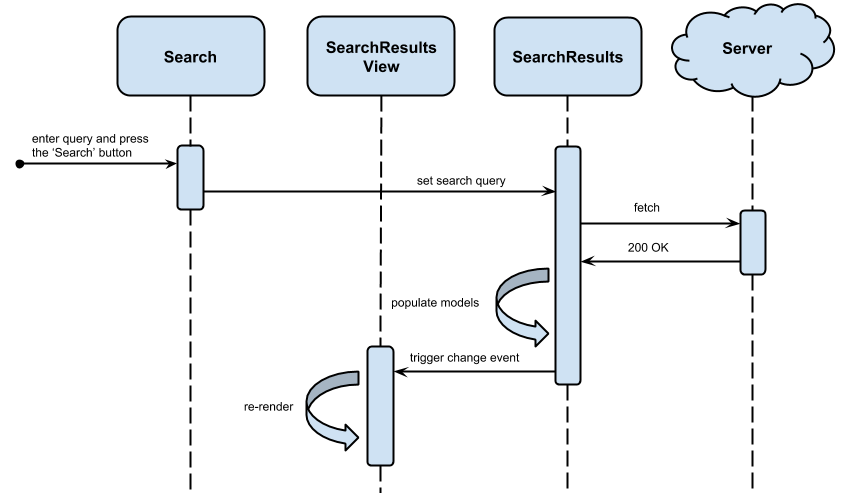
\includegraphics[width=1\textwidth]{web_system_sequenceDiagram.png}
\caption{\label{fig:web_system_sequenceDiagram}a sequence diagram showing what happens when a user enters a valid search query and results are fetched.}
\end{figure}

In \refer{fig:web_system_sequenceDiagram} is a simple sequence diagram for the search tab. If a user enters a query in the search field and then presses the search button, the \textit{Search} view will update the \textit{SearchResults} collection to have a new query. Once \textit{SearchResults} has a new query, it will try to fetch search results corresponding to the query from the server. If successful, new experiment models for every experiment retrieved will be created and set in the \textit{SearchResults} collection. \textit{SearchResults} then triggers a ‘change’ event that \textit{SearchResultsView} listens to. When that event occurs, \textit{SearchResultsView} knows that \textit{SearchResults} has been changed, and re-renders itself.


\subsection{Upload}
The upload tab has three main views, the main one being Upload, which acts as a container for the ExperimentView’s and holds the search input field and the various buttons displayed. Each ExperimentView handles rendering the AnnotationsForm and the FileUploadList, where one ExperimentView is created for every experiment the user inputs. The actual annotation data is stored by the \textit{Experiment} model. Files are stored as a \textit{Files} collection in the \textit{Experiment} model. \textit{Experiments} are in turn stored in the \textit{Experiments} collection.
\subsection{Process}
Processing has genomeReferences to match with the specie the processing is being done on. Other that that the processing part is mainly a graphical interface with not that much systemDesgin in.
